\documentclass{exam}
\usepackage[fontsize=12pt]{scrextend}
\usepackage{xpatch}
\usepackage{babel}
\usepackage{graphicx}
\usepackage{float}  % Added to support the H option in figures

\pointsdroppedatright
\marksnotpoints
\makeatletter
\def\mydroppoints{%
  {\unskip\nobreak\hfil\penalty50
    \hskip2em\hbox{}\nobreak\hfil
    (\@points~mark\expandafter\ifx\@points1\else s\fi)
    \parfillskip=0pt \finalhyphendemerits=0 \par}
}
\makeatother

\usepackage{geometry}
\geometry{
  a4paper,% redundant if already in \documentclass
  left=25mm,
  right=25mm,
  top=25mm,
  bottom=25mm,
  heightrounded,% better use it
}

\begin{document}

\begin{center}
\textbf{CS300: Computer Networks(2023--24--M)} \\
\textbf{Assignment}
\end{center}

\vspace{0.2in}

\noindent
\textsc{\textbf{Full name : Munjam Navadeep}}  \hspace{1in} \textsc{\textbf{ID: 12241060}}

\vspace{0.2in}


\section*{Question 1}



\begin{figure}[H]
    \centering
    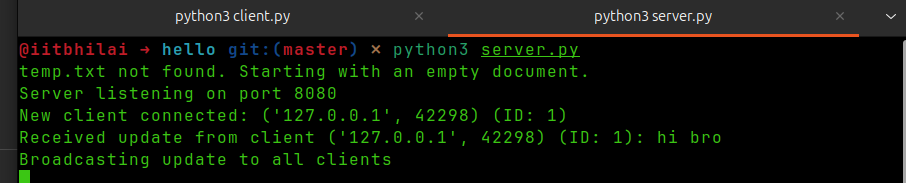
\includegraphics[width=0.9\textwidth]{1stQ.png } 
    \caption{ output when no temp.txt file is present }
    \label{fig:output1}
\end{figure}


\begin{enumerate}
    \item \textbf{Socket Setup and Connection}:
    \begin{itemize}
        \item \texttt{HOST} and \texttt{PORT} define the server address (\texttt{'localhost'}) and port (8080) for the connection.
        \item \texttt{client\_socket = socket.socket(socket.AF\_INET, socket.SOCK\_STREAM)} This actually creates a TCP connection
        \item \texttt{client\_socket.connect((HOST, PORT))} 
        It will try to establish a connection with server on specified host and specified port
    \end{itemize}
    
    \item \textbf{Receiving Updates}:
    \begin{itemize}
        \item The function \texttt{for\_receiving\_The\_updates(sock)} 
        will run in a separate thread so that it can continuously receive updates from the server.
        
        
        \item First it reads a header (10 bytes)  which it is length of incoming message from client
    
        \item The function retrieves the actual message content based on the length indicated by the header using \texttt{sock.recv(updated\_the\_length)}.
        \item
        If the data is not received or if any error occurs the  loop automatically terminates and exits.
    \end{itemize}
    
    \item \textbf{Thread for Asynchronous Reception}:
    \begin{itemize}
        \item A new thread is created using Python's \texttt{threading.Thread} class to run \\ \texttt{for\_receiving\_The\_updates}. 
        this helps the client to send messages and receive messages simultaneously without blocking anything.
    \end{itemize}
    
    \item \textbf{Sending Updates}:
    \begin{itemize}
        \item In the main loop, the client waits for user input using \texttt{input()}.
        \item The message is formatted by prepending the length of the message  to enable the server to correctly read and process the data.
        \item The combined message (\texttt{message = f"\{len(update):<10\}" + update}) is sent over the network using \texttt{client\_socket.sendall(message.encode())}.
    \end{itemize}
    
    \item \textbf{Error Handling}:
    \begin{itemize}
        \item Basic error-handling mechanisms are in place to manage issues with connection and data transmission, providing error messages in case of failures.
    \end{itemize}
\end{enumerate}


\begin{figure}[H]
    \centering
    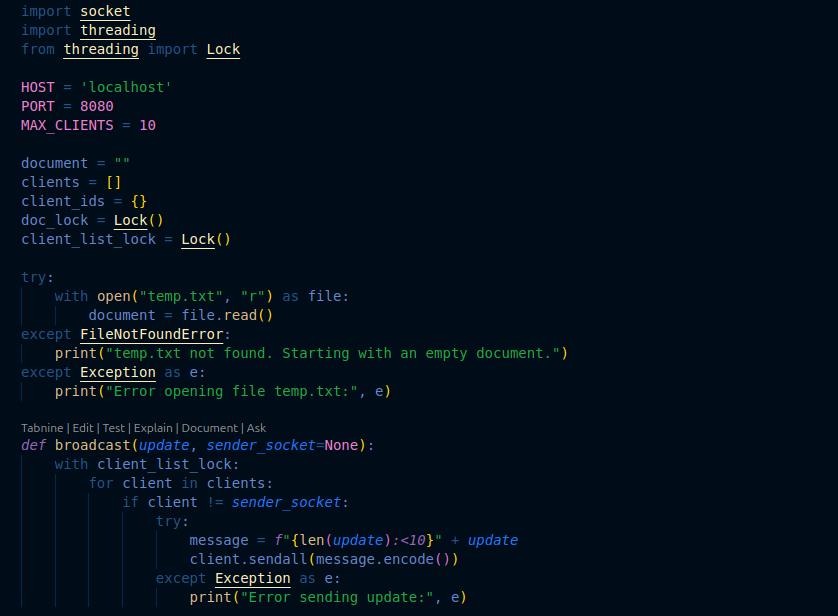
\includegraphics[width=0.9\textwidth]{Q1_server_starting_code.png } 
    \caption{server code}
    \label{fig:output1}
\end{figure}


\begin{figure}[H]
    \centering
    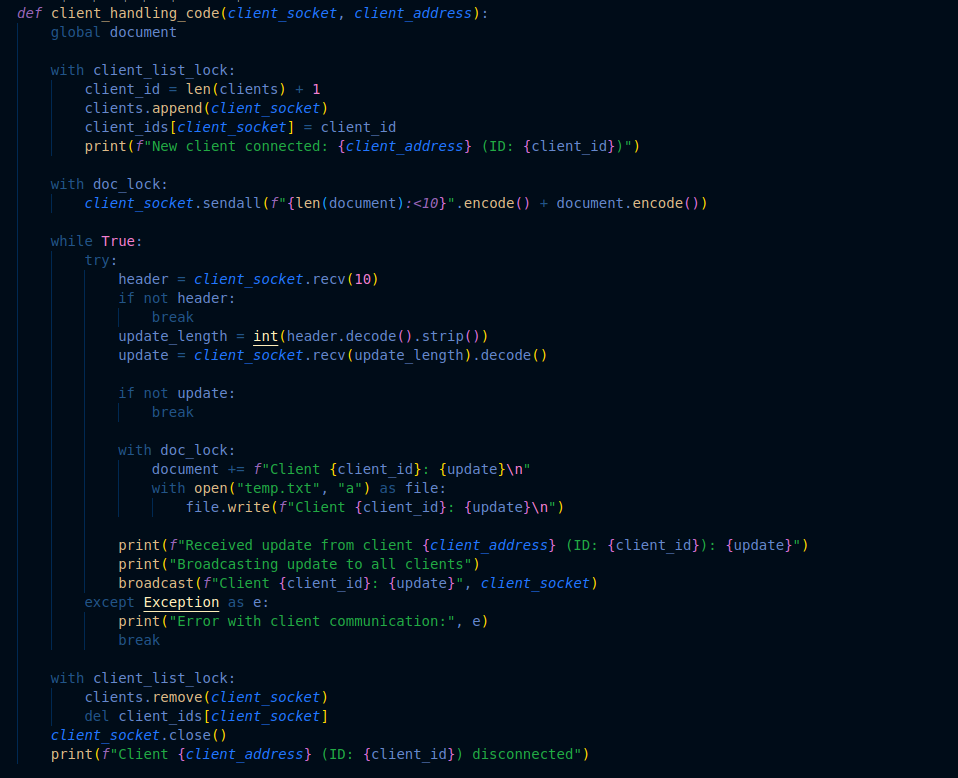
\includegraphics[width=0.9\textwidth]{Q1_handling_client_Code.png } 
    \caption{ client handling function code}
    \label{fig:output1}
\end{figure}




\begin{figure}[H]
    \centering
    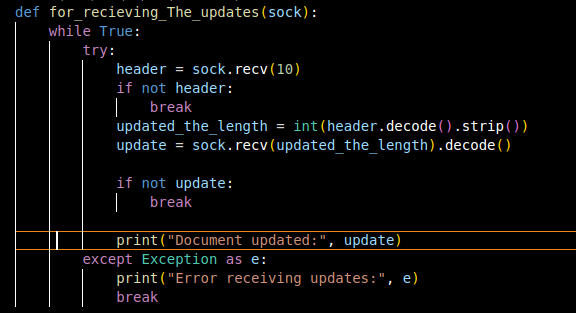
\includegraphics[width=0.78\textwidth]{update_Receive.png } 
    \caption{client code}
    \label{fig:output1}
\end{figure}

\begin{figure}[H]
    \centering
    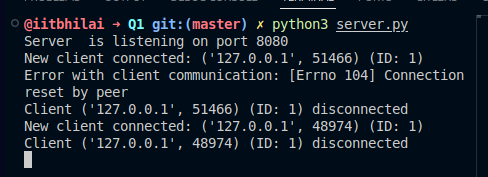
\includegraphics[width=0.9\textwidth]{Q1_connection.png } 
    \caption{connection-disconnection output}
    \label{fig:output1}
\end{figure}

\begin{figure}[H]
    \centering
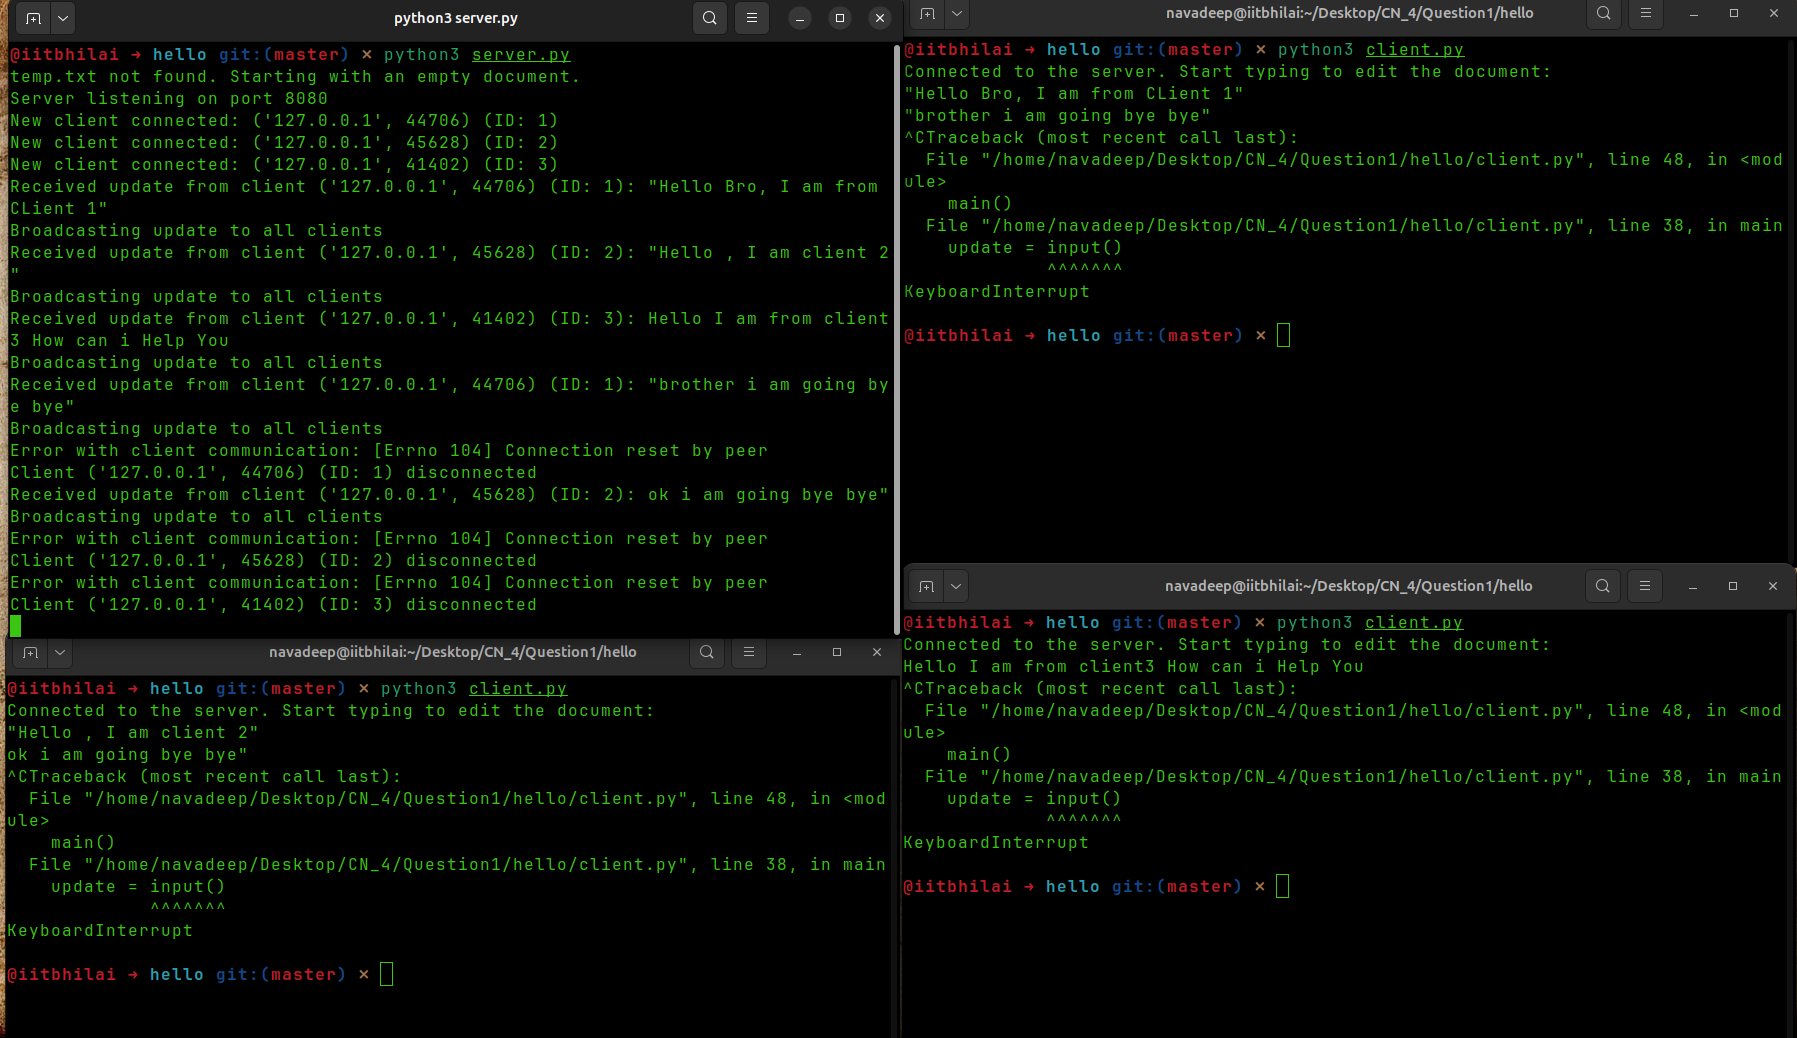
\includegraphics[width=0.9\textwidth]{Q1output.png } 
    \caption{Output for question 1}
    \label{fig:output1}
\end{figure}


\section*{Server Responsibilities}

\begin{enumerate}
    \item \textbf{Listen for Incoming Client Connections:} 
    
    
    The server listens on a specific port (8080) for incoming client connections. It handles up to 10 clients concurrently by spawning a new thread for each client.
    \item \textbf{Manage a Shared Document:} The server maintains the document in memory, which is shared among all connected clients. It holds the current state of the document and is responsible for broadcasting any updates to all connected clients.
    \item \textbf{Handle Concurrent Edits:} The server uses synchronization mechanisms such as mutex locks to ensure that the document is edited safely, preventing race conditions when multiple clients attempt to update the document at the same time.
    \item \textbf{Broadcast Updates:} When a client sends an update, the server appends the change to the document in memory and saves it to \texttt{temp.txt} to ensure persistence. It then broadcasts the update to all other connected clients.
    \item \textbf{Persist Document Changes:} All document updates are appended to the \texttt{temp.txt} file to ensure that the document is saved and can be restored in case the server stops or restarts.
    \item \textbf{Handle Client Disconnects:} When a client disconnects, the server removes the client from the active list and prints the client's disconnection message.
\end{enumerate}

\subsection*{Server Error Handling}
The server handles errors in the following scenarios:
\begin{itemize}
    \item \textbf{Server Startup Errors:} If the server cannot create or bind the socket to port 8080, it prints an error message: \texttt{"Server error: Unable to start server on port 8080"}.
    \item \textbf{File Access Errors:} If there is an issue opening the \texttt{temp.txt} file for writing, the server prints: \texttt{"Error opening file temp.txt"}.
\end{itemize}

\section{Client Responsibilities}
The client performs the following tasks to interact with the server and contribute to the collaborative editing process:

\begin{enumerate}
    \item \textbf{Connect to the Server:} The client attempts to connect to the server using the server's IP address and port (8080). Upon successful connection, the client prints: \texttt{"Connected to the server. Start typing to edit the document:"}.
    \item \textbf{Receive Document Updates:} The client continuously listens for updates from the server. When a new update is received, the client prints: \texttt{"Document updated: <received\_content>"} to display the latest version of the document.
    \item \textbf{Send Edits to the Server:} The client allows the user to input text to edit the document. The client sends the edited text back to the server for processing and broadcasting to other clients.
\end{enumerate}

\subsection*{Client Error Handling}
The client handles errors such as connection failures. If the client cannot connect to the server, it displays: \texttt{"Connection failed. Please check the server and try again."}

\section*{Concurrency and Synchronization}
\begin{itemize}
        \item \textbf{Concurrency:} The server handles multiple client connections concurrently by spawning a new thread for each client. Each client can independently send updates and receive changes without blocking other clients. This enables multiple users to edit the document simultaneously.
    \item \textbf{Synchronization:} To prevent data inconsistencies, the server uses \textit{mutex locks} to synchronize access to the shared document. This ensures that only one client can update the document at any given time, preventing race conditions and ensuring data integrity.
\end{itemize}

\section*{Document Persistence}
To ensure the document persists even if the server crashes or restarts:
\begin{itemize}
    \item Each update from the client is appended to a file named \texttt{temp.txt}.
    \item On server restart, the server can load the contents of \texttt{temp.txt} to restore the document to its last saved state.
\end{itemize}

\section*{Message Flow}
\begin{enumerate}
    \item \textbf{Server Starts:} The server listens on port 8080. If successful, it prints \texttt{"Server listening on port 8080"}.
    \item \textbf{Client Connects:} A client connects to the server, and the server sends the current state of the document.
    \item \textbf{Client Edits and Sends Updates:} The client makes edits and sends the updated text to the server. The server processes the update, saves it to \texttt{temp.txt}, and broadcasts it to all connected clients.
    \item \textbf{Clients Receive Updates:} All clients receive the broadcasted update and display the new version of the document.
\end{enumerate}
\newpage


\section*{ Question 2}

Note : In this  Question 2 folder there 
The server will on listen for incoming TCP connections on port \texttt{12345}. 
It is used to handle both \texttt{IPv4} and \texttt{IPv6} addresses. 

The server runs asynchronously, means that  it can accept and handle multiple client connections simultaneously without blocking.

\section*{Client Handling}
When a client connects, the server assigns a coroutine to manage that connection.
The \texttt{asyncio} library ensures that the server can handle multiple clients concurrently, so that itcan allow  to read from and write to clients in a non-blocking manner. 
This avoids delays, as the server does not wait for one client to finish before serving the next.

\section*{Reading and Writing Data}
Once the  client is connected, the server reads data sent by the client, it will logs the received message, and then sends the same data back to the client (echoing it). 
The reading and writing of data is done asynchronously, which means the server doesn’t block waiting for data. It can continue handling other tasks while waiting for input or output operations to complete.

\section*{Logging}
Throughout the server's operation, various events are logged using Python's \texttt{logging} module. This includes:
\begin{itemize}
    \item When a client connects.
    \item The data received from the client.
    \item The data sent back (echoed) to the client.
    \item Any errors or unexpected events that occur during communication.
\end{itemize}

\section*{Connection Management}
The server will continue to handle communication with clients until the client disconnects or sends no data. If any error occurs, the server logs the error and gracefully closes the connection with the client. It ensures proper cleanup and avoids leaving open connections.

\section*{Asynchronous Execution}
The core of the server is built around \texttt{asyncio}, which allows it to perform asynchronous operations. This means the server is capable of handling multiple clients simultaneously:
\begin{itemize}
    \item It reads and writes data to clients asynchronously, meaning it does not block or wait for one client to finish before serving another.
    \item The \texttt{await} keyword is used to pause the execution of a task until it is completed, allowing the server to switch between tasks efficiently without blocking other tasks.
\end{itemize}

\section*{Key Features}
The server is designed with the following key features:
\begin{itemize}
    \item \textbf{Non-blocking behavior}: It means that the server can handle multiple clients at the same time without blocking.
    \item \textbf{Echo server}: The server simply echoes back whatever message that client sends.
    \item \textbf{Logging}: Every action taken by the server is logged, like the  incoming connections and data exchanges.
    \item \textbf{Graceful shutdown}: The server handles errors and ensures  thst connections are properly closed.
\end{itemize}
\begin{figure}[H]
    \centering
    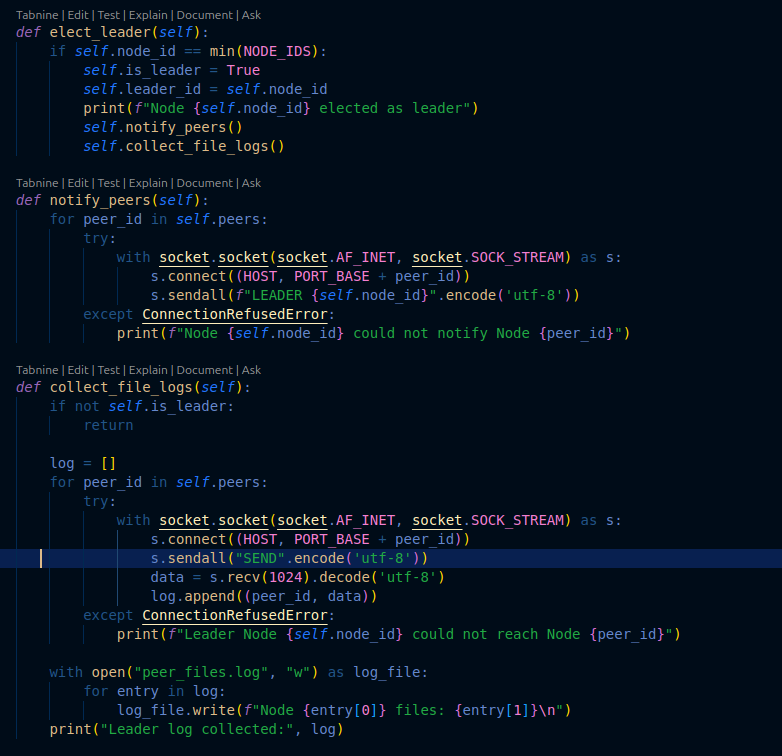
\includegraphics[width=0.9\textwidth]{Q2_1.png } 
    \caption{Output for question 2}
    \label{fig:output1}
\end{figure}
\begin{figure}[H]
    \centering
    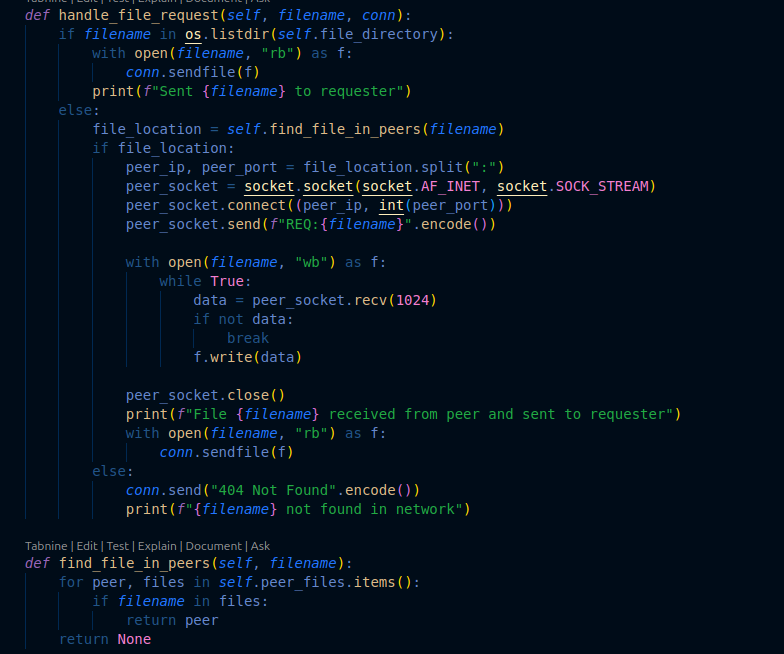
\includegraphics[width=0.9\textwidth]{Q21.png } 
    \caption{Output for question 2}
    \label{fig:output1}
\end{figure}

\begin{figure}[H]
    \centering
    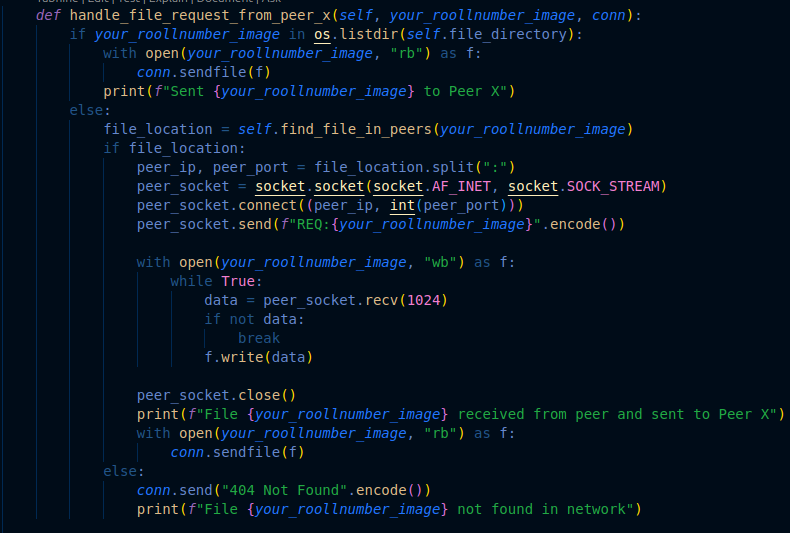
\includegraphics[width=0.9\textwidth]{Q2_2question.png } 
    \caption{question 2 part 2 code}
    \label{fig:output1}
\end{figure}

    \item \textbf{File Transfer:}
    \begin{itemize}
        \item If Peer Y hosts the file, then the  leader requests for  file from Peer Y and it will forwards it to Peer X.
        \item when the leader hosts the file, then it directly sends it to Peer X.
        \item If the file is not found, the leader responds with \texttt{404 Not Found}.
    \end{itemize}
    \item \textbf{Concurrency:} Multi-threading used to handle  files simentenuously
\end{enumerate}


\begin{figure}[H]
    \centering
    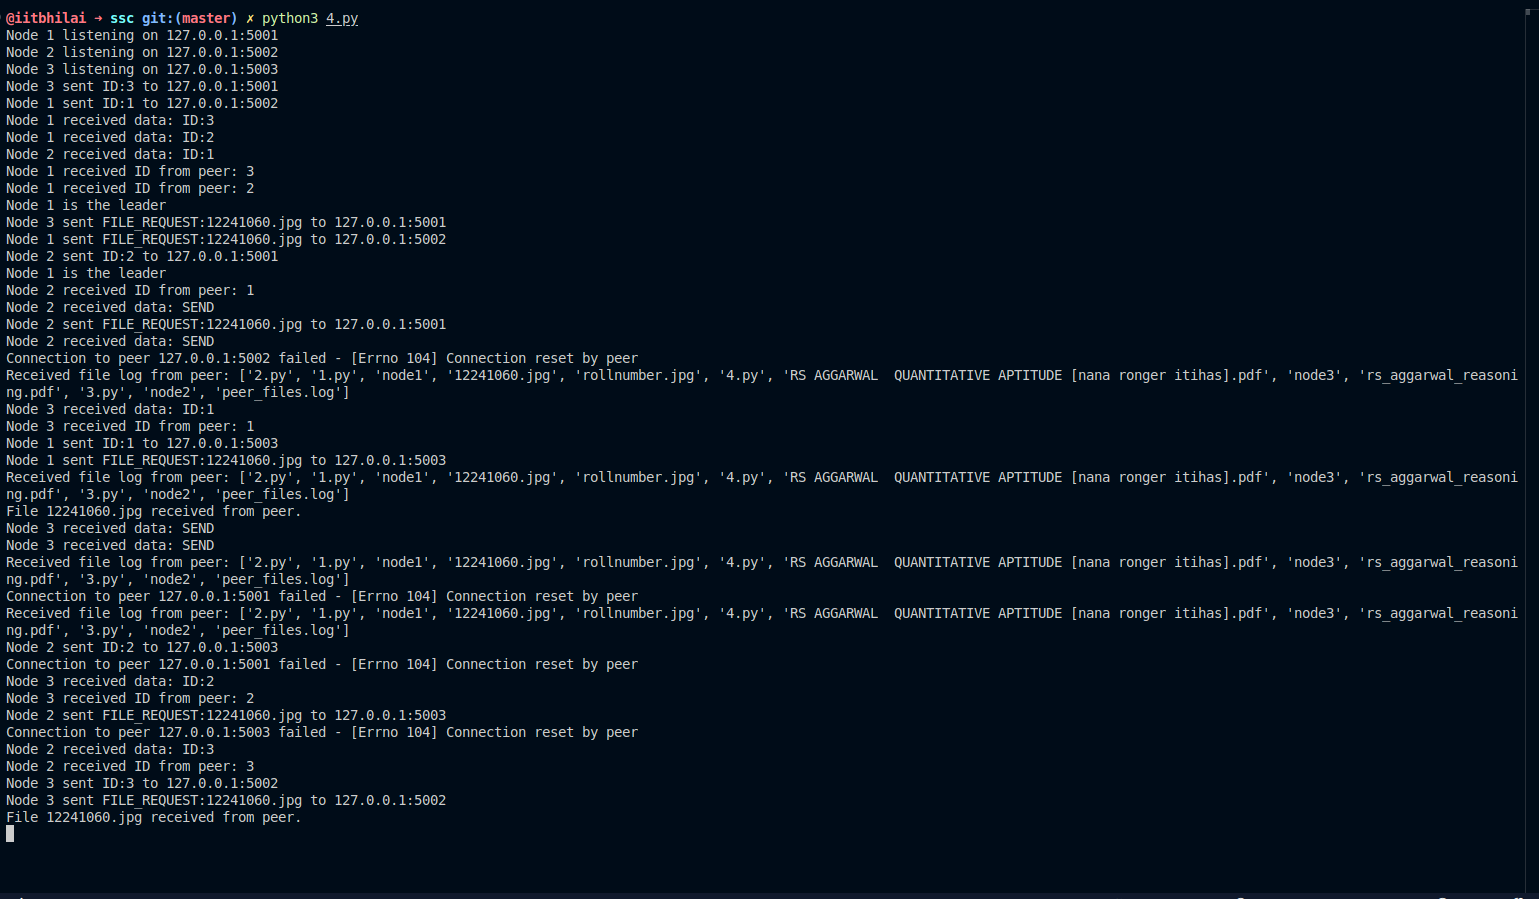
\includegraphics[width=1.1\textwidth]{Q2final_output.png } 
    \caption{Final output for whole question 2}
    \label{fig:output1}
\end{figure}
\newpage
\section*{Question 3 }

\begin{enumerate}
    \item \textbf{Imports and Logging Configuration}:
    \begin{itemize}
        \item In client code we will  imports the \texttt{asyncio}, \texttt{socket}, and \texttt{logging} modules.
        \item Logging is configured using \texttt{lg.basicConfig} with a log level of \texttt{INFO} and a simple format.
    \end{itemize}
    
    \item \textbf{\texttt{client\_echo\_using\_tcp} Coroutine}:
    \begin{itemize}
        \item 
        This one is main synchronous function which is useful for handling the TCP connection
        \item \textbf{Host, Port, and Protocol}:
        \begin{itemize}
            \item The user specifies the server's \texttt{host} and \texttt{port}.
            \item The \texttt{protocol} parameter defaults to \texttt{ipv4}, but if user want to choose   \texttt{ipv6} then using ip6-localhost they can do.
        \end{itemize}
        \item \textbf{Address Information Resolution}:
        \begin{itemize}
            \item Depending on the protocol, \texttt{socket.getaddrinfo} retrieves address information. \texttt{AF\_INET} and \texttt{AF\_INET6} specify IPv4 and IPv6 families respectively.
        \end{itemize}
        \item \textbf{Attempting Connection}:
        \begin{itemize}
            \item This function iterates all the  addresses returned by \texttt{getaddrinfo}.
            \item first it  tries to open a connection using \texttt{asyncio.open\_connection}.
            \item Upon success, it logs the connection establishment.
            \item If a connection fails, then it tries to attempts to use other addresses until all options are exhausted.
        \end{itemize}
    \end{itemize}
    
    \item \textbf{Message Sending and Receiving Loop}:
    \begin{itemize}
        \item The client enters a loop, accepting the user input: \begin{itemize}
            \item If the user want to exit from that server then if they  types ``exit'', the loop terminates and the connection closes.
            \item Otherwise, the input message is encoded and sent to the server using \texttt{writer.write()}.
            \item The \texttt{await writer.drain()} ensures data is flushed through the socket.
        \end{itemize}
        \item The client then waits to receive a response using \texttt{await reader.read(1024)} and logs the received data.
        \item The loop continues until the user decides to exit.
    \end{itemize}
    
    \item \textbf{Error Handling}:
    \begin{itemize}
        \item The code handles \texttt{ConnectionRefusedError} and \texttt{OSError} to manage connection issues and retries other addresses as needed.
        \item It will handle all the errors mentioned in the question.
    \end{itemize}
\end{enumerate}

\subsection*{User Input and Script Execution}
In final part of code it prompts the user for the server's IP address, port, and protocol type. The function \texttt{aio.run(client\_echo\_using\_tcp(host, port, protocol))} runs the asynchronous client function.

\subsection*{Asynchronous Operation}
\begin{itemize}
    \item The \texttt{asyncio} library enables non-blocking I/O, allowing the client to send and receive messages asynchronously.
    \item The use of \texttt{await} pauses the execution until runs after the data gets it will resume it progress.
\end{itemize}

\begin{figure}[H]
    \centering
    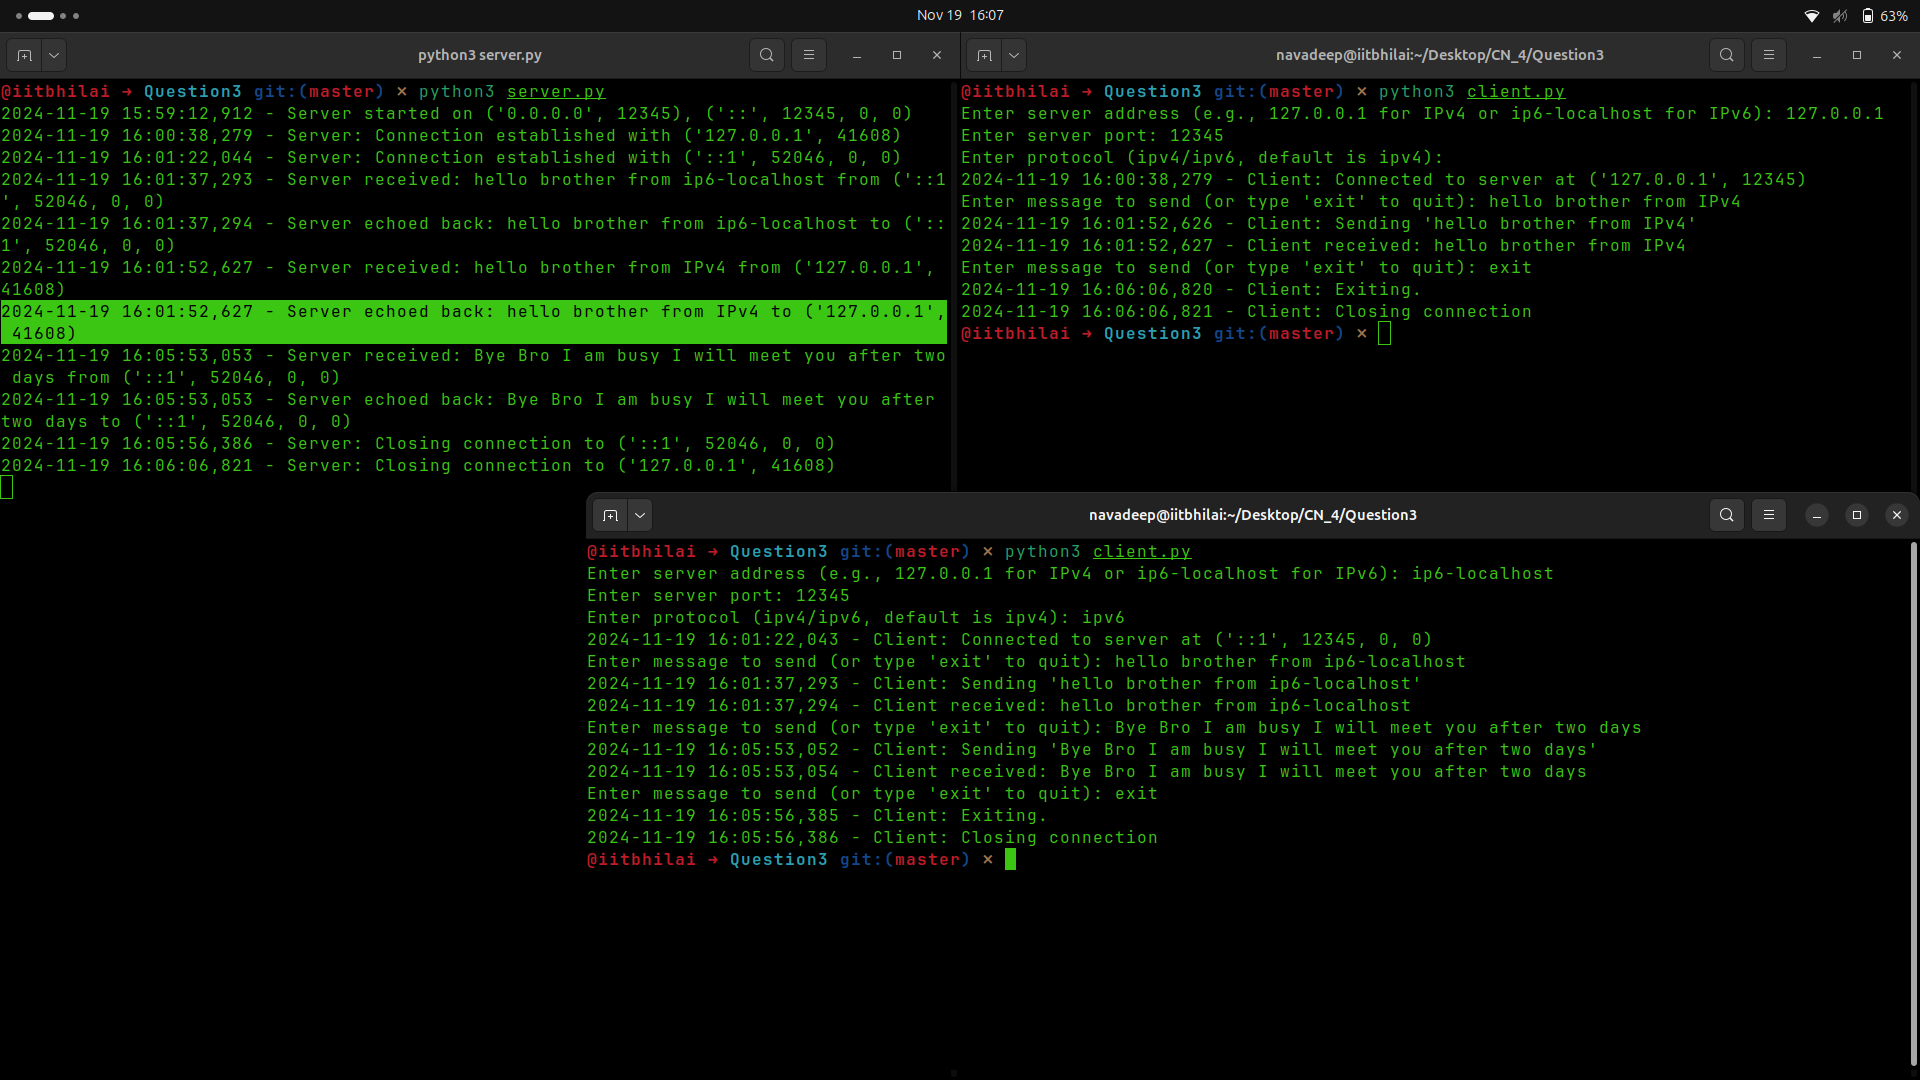
\includegraphics[width=0.98\textwidth]{3rd_Output.png} % Specify image file name and optional parameters for size
    \caption{Output for third scenario}
    \label{fig:output2}
\end{figure}


\newpage

\begin{figure}[H]
    \centering
    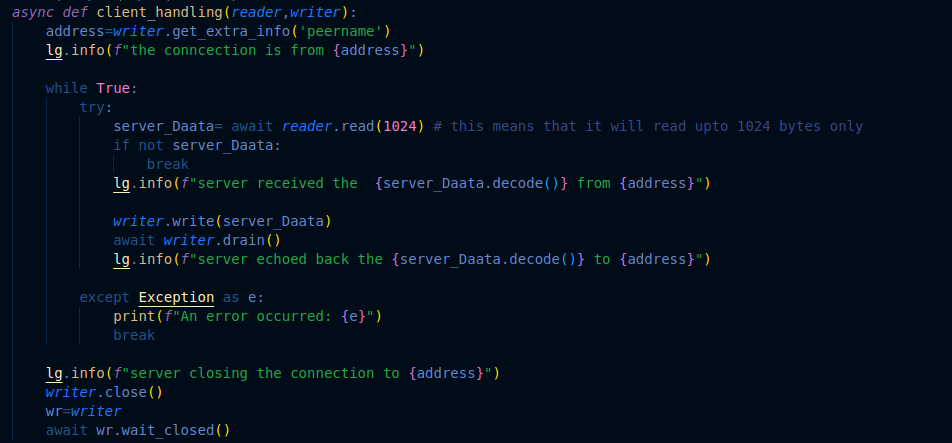
\includegraphics[width=0.9\textwidth]{Q3_clienthandling_server.png} % Specify image file name and optional parameters for size
    \caption{function code using client\_handling}
    \label{fig:output2}
\end{figure}

\begin{figure}[H]
    \centering
    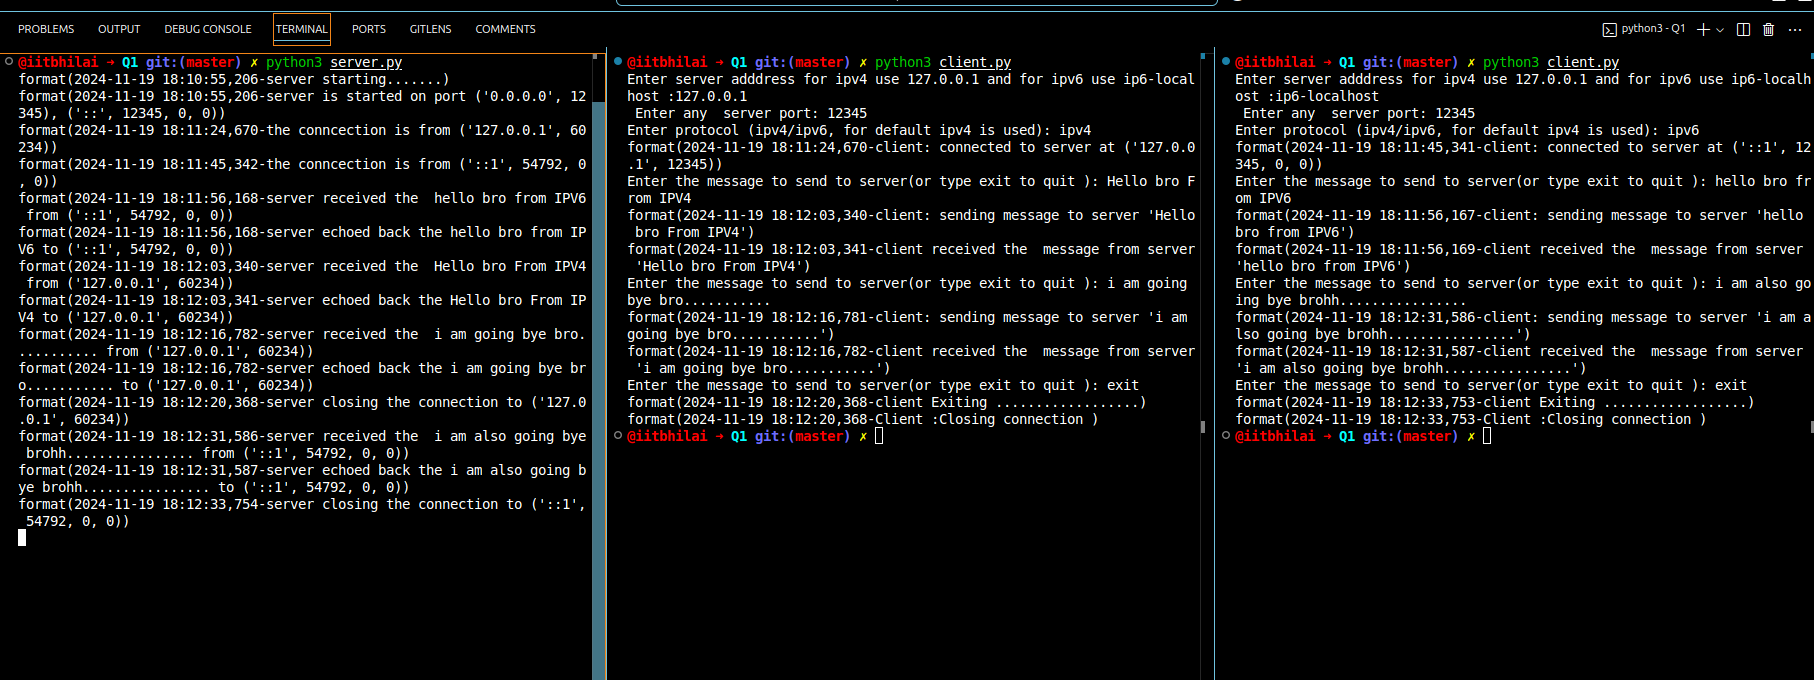
\includegraphics[width=0.9\textwidth]{Q3finaloutput.png } 
    \caption{Final output  fror Question 3 }
    \label{fig:output1}
\end{figure}

This function \texttt{client\_handling} is an asynchronous server-side handler.It is used to manage client connections. 
\begin{enumerate}
    \item \textbf{Accepting and Logging the Client Connection:}
    \begin{itemize}
        \item The function retrieves the address (IP and port) of the client that has connected using \texttt{writer.get\_extra\_info('peername')}.
        \item The server logs the client's address, allowing it to track the origin of the connection.
    \end{itemize}
    
    \item \textbf{Continuous Listening for Data:}
    \begin{itemize}
        \item The function enters an infinite loop with \texttt{while True} to continuously listen for data from the client.
        \item It reads up to 1024 bytes of incoming data from the client using \texttt{await reader.read(1024)}.
    \end{itemize}
    
    \item \textbf{Processing the Received Data:}
    \begin{itemize}
        \item When the server  receives data successfully, then it will decodes the byte data into a string.
        \item The server logs the received data for debugging .
    \end{itemize}
    
    \item \textbf{Echoing the Data Back to the Client:}
    \begin{itemize}
        \item After processing the data, the server immediately sends the exact same data back to the client (echoes it) using \texttt{writer.write(server\_data)}.
        \item The function waits for the data to be fully written to the client with \texttt{await writer.drain()}, ensuring no data is lost.
    \end{itemize}
    
    \item \textbf{Handling Errors:}
    \begin{itemize}
        \item 
        I used try ,expect method for if any error occurs during data writing or reading then this expect will handle the errors. 
        \item The error message will be printed , and the  loop will break and connection is closed .
    \end{itemize}
    
    \item \textbf{Closing the Connection:}
    \begin{itemize}
        \item Once the loop terminates (due to client disconnection or an error), then server logs that it is closing the connection.
        \item The server then calls \texttt{writer.close()} to close the connection and waits for the closure to complete with \texttt{await writer.wait\_closed()}.
    \end{itemize}
\end{enumerate}

\end{document}
